\documentclass[10pt]{beamer}

\newcommand{\lectnum}{L04}
\newcommand{\lecttitle}{Linear Regresssion, Linear Discriminant and
  Logistic Regression}

\usepackage{amsmath, amssymb, graphicx}
\usepackage[]{algorithm2e}
\usepackage{pdfpages}
\usepackage[british]{babel}

\hypersetup{colorlinks,linkcolor=,urlcolor=blue}
\newenvironment{titledslide}[1]{\begin{frame}\frametitle{#1}}{\end{frame}}

\mode<presentation>{\setbeamercovered{transparent}}

\setbeamertemplate{sidebar right}{}
\setbeamertemplate{footline}{%
\hfill\usebeamertemplate***{navigation symbols}
\hspace{0.4cm}\lectnum: \insertframenumber{}/\inserttotalframenumber \hspace*{0.4cm}}

\author{James Cussens}

\title{COMS30035, Machine learning:\\ \vspace{5pt} \lecttitle}

\institute{School of Computer Science\\University of Bristol}

\begin{document}
%%%%%%%%%%%%%%%%%%%%%%%%%%%%%%%%%%%%%%%%%%%%%%%%%%%%%%%%%%%%%%%%%%%%%%

\begin{frame}
  \titlepage
\end{frame}

%%%%%%%%%%%%%%%%%%%%%%%%%%%%%%%%%%%%%%%%%%%%%%%%%%%%%%%%%%%%%%%%%%%%%%


%%%%%%%%%%%%%%%%%%%%%%%%%%%%%%%%%%%%%%%%%%%%%%%%%%%%%%%%%%%%%%%%%%%%%%
\begin{titledslide}{Acknowledgement}

  \begin{itemize}
  \item These slides are adapted from ones originally created by
    \href{https://www.dpag.ox.ac.uk/team/rui-ponte-costa}{Rui Ponte
      Costa} and Dima Damen and later edited by Edwin Simpson. 
  \end{itemize}
  
\end{titledslide}
%%%%%%%%%%%%%%%%%%%%%%%%%%%%%%%%%%%%%%%%%%%%%%%%%%%%%%%%%%%%%%%%%%%%%%
\begin{frame}[fragile]

  \frametitle{Textbooks}
  Chapter 3 of the Bishop book is directly relevant:
  \begin{itemize}
  \item Bishop, C. M., Pattern recognition and machine learning (2006). Available for free \href{https://www.microsoft.com/en-us/research/people/cmbishop/prml-book/}{here.}	\vspace{10pt}
  \item \textbf{Note:} this first part is a revision of should be
    covered in Data-driven Computer Science in your 2nd year.
\end{itemize}

\end{frame}
%%%%%%%%%%%%%%%%%%%%%%%%%%%%%%%%%%%%%%%%%%%%%%%%%%%%%%%%%%%%%%%%%%%%%%

\begin{frame}[fragile]
\frametitle{Agenda}
\begin{itemize}
		\item Linear regression
		\item Nonlinear regression		
		\item Probabilistic models
		\item Maximum likelihood estimation
\end{itemize}

\end{frame}
%%%%%%%%%%%%%%%%%%%%%%%%%%%%%%%%%%%%%%%%%%%%%%%%%%%%%%%%%%%%%%%%%%%%%%
\begin{frame}[fragile]
\frametitle{Revisiting regression}

\begin{itemize}
\item Goal: Finding a relationship between two variables \begin{small}(e.g. regress \emph{house value} against \emph{number of rooms})\end{small}
\vspace{12pt}
\item Model: Linear relationship between \emph{house value} and \emph{number of rooms}?
\end{itemize}
\vspace{6pt}
\centerline{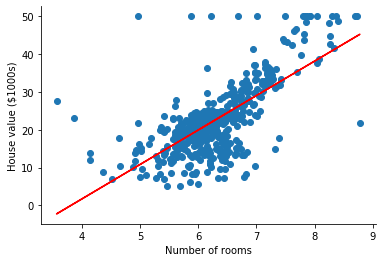
\includegraphics[scale=0.5]{../figures/boston_linear1.png}}
\end{frame}


%%%%%%%%%%%%%%%%%%%%%%%%%%%%%%%%%%%%%%%%%%%%%%%%%%%%%%%%%%%%%%%%%%%%%%
\begin{frame}[fragile]
  
\frametitle{Revisiting regression -- deterministic model}

\textbf{\textcolor{blue}{Data:}} a set of data points $D = \{ (x_1, y_1), (x_2, y_2), \cdots, (x_N, y_N) \}$ where $x_i$ is the number of rooms of house $i$ and $y_i$ the house value.
\vspace{6pt}

\textbf{\textcolor{blue}{Task:}} build a model that can predict the house value from the number of rooms
\vspace{6pt}

\uncover<2->{\textbf{\textcolor{red}{Model Type:}} parametric; assumes a polynomial relationship between house value and number of rooms}
\vspace{6pt}

\uncover<3->{\textbf{\textcolor{red}{Model Complexity:}} assume the relationship is linear $\text{house value} = a_0 + a_1 \times \text{rooms}$
\begin{equation}
y_i = a_0 + a_1 x_i
\end{equation}}
\vspace{6pt}

\uncover<4->{\textbf{\textcolor{red}{Model Parameters:}} model has two parameters $a_0$ and $a_1$ which should be estimated.

\begin{itemize}
\item $a_0$ is the y-intercept
\item $a_1$ is the slope of the line
\end{itemize}}

\end{frame}
%%%%%%%%%%%%%%%%%%%%%%%%%%%%%%%%%%%%%%%%%%%%%%%%%%%%%%%%%%%%%%%%%%%%%%
\begin{frame}[fragile]
  
\frametitle{Revisiting linear regression -- fitting}

\begin{itemize}
\item Although we are currently assuming the model is linear, the data
  will not typically be consistent with such an assumption. So \dots
\item Find $\theta=(a_{0},a_{1})$ which minimises 
\begin{equation}
R(a_{0},a_{1}) = \sum_{i=1}^N {(y_i - (a_{0} + a_{1}x_i))^2}
\end{equation}
\item This is the \textcolor{blue}{sum of squared residuals}.
\item Using matrix notation we have:
\end{itemize}

\[
  \frac{\partial R}{\partial \theta} = -2\mathbf{X}^{T}(\mathbf{y}-\mathbf{X}\theta)
\]

\begin{itemize}
\item Here $X_{i,j}$ is the value of the $j$th feature in the $i$th
  datapoint (where we add a fake feature which is always 1 to handle
  the intercept), and $y_i$ is the value of the \emph{response} in the
  $i$th datapoint.
\item Setting $\frac{\partial R}{\partial \theta}$ to 0 and
  re-arranging we get:
\end{itemize}

\[
  \hat{\theta} = (\mathbf{X}^T \mathbf{X})^{-1}\mathbf{X}^T\mathbf{y}
\]


\end{frame}
%%%%%%%%%%%%%%%%%%%%%%%%%%%%%%%%%%%%%%%%%%%%%%%%%%%%%%%%%%%%%%%%%%%%%% 
\begin{frame}[fragile]
  
  \frametitle{Linear regression for nonlinear models}
  
  \begin{itemize}
  \item For a polynomial of degree $p+1$ we use \begin{tiny}(note:
      $p>1$ gives nonlinear regression)\end{tiny}
  \end{itemize}

  \begin{equation}
    y_i = a_0 + a_1 x_i + a_2 x_i^2 + \cdots + a_{p} \ x_{i}^{p} 
  \end{equation}
  

\end{frame}
%%%%%%%%%%%%%%%%%%%%%%%%%%%%%%%%%%%%%%%%%%%%%%%%%%%%%%%%%%%%%%%%%%%%%%
\begin{frame}[fragile]
\frametitle{Least Squares Solution}
\begin{example}
Find the best least squares fit by a linear function to the data using $p=1$

\begin{center}
\begin{tabular}{c|c|c|c|c}
x &-1 &0 &1 &2\\ \hline
y &0 &1 &3 &9
\end{tabular}
\end{center}
\end{example}

\uncover<2->{$\textbf{y} = \begin{bmatrix} 0\\ 1\\ 3\\ 9 \end{bmatrix}$} \hspace{6pt} \uncover<3->{$\textbf{X} = \begin{bmatrix} 1 &-1\\ 1&0\\ 1 &1\\ 1 &2 \end{bmatrix}$}
\hspace{6pt} \uncover<4->{$\textbf{X}^T \textbf{X} = \begin{bmatrix} 1 &1 &1 &1\\ -1 &0 &1 &2 \end{bmatrix} \begin{bmatrix} 1 &-1\\ 1&0\\ 1 &1\\ 1 &2 \end{bmatrix} = \begin{bmatrix} 4 &2\\ 2 &6\end{bmatrix}$}\\
\vspace{6pt}

\uncover<5->{$\hat{\theta} = (\textbf{X}^T \textbf{X})^{-1} \textbf{X}^T \textbf{y}$} \uncover<6->{$= \frac{1}{20} \begin{bmatrix} 6 &-2\\ -2 &4 \end{bmatrix}$} \uncover<7->{$\begin{bmatrix} 1 &1 &1 &1\\ -1 &0 &1 &2 \end{bmatrix}$} \uncover<8->{$\begin{bmatrix} 0\\ 1\\ 3\\ 9 \end{bmatrix}$} \uncover<9->{$= \begin{bmatrix} 1.8\\ 2.9 \end{bmatrix}$}

\uncover<10->{$y = 1.8 + 2.9 x$}
\end{frame}




\begin{frame}[fragile]
\frametitle{Regression with probabilistic models}

\begin{small}\textbf{Probabilistic models are a core part of ML}, as they allow us to also capture the uncertainty the model has about the data, which is critical for real world applications. For simplicity, lets drop $a_0$ from the previous model and add a random variable $\epsilon$ that captures the uncertainty \end{small}
\begin{equation*}
\text{house price} = a_1 \times \text{number of rooms} + \epsilon
\end{equation*}


\uncover<2->{We can assume, for example, that $\epsilon$ is given by $\mathcal{N}(\mu=0, \sigma^2)$ which gives the likelihood
\begin{align*}
p(\textbf{y}|\textbf{X},\theta) &= \prod\limits_{i=1}^N{p(\text{price}_i | \text{rooms}_i, \theta)} = \prod\limits_{i=1}^N {\frac{1}{\sqrt{2 \pi} \sigma} e^{-\frac{1}{2}\frac{(\text{price}_i - a_1\text{rooms}_i)^2}{\sigma^2}}}
\end{align*}}

%\begin{equation*}
%p(\epsilon) = \frac{1}{\sqrt{2 \pi} \sigma} e^{-\frac{\epsilon^2}{2 \sigma^2}}
%\end{equation*}}

\uncover<3->{\small This model has \textcolor{red}{two} parameters: the slope $a_1$ and variance $\sigma$ \footnote{\tiny Note that here $\mu = a_0$ which, for simplicity, we assume to be zero.}
\vspace{0pt}

\centerline{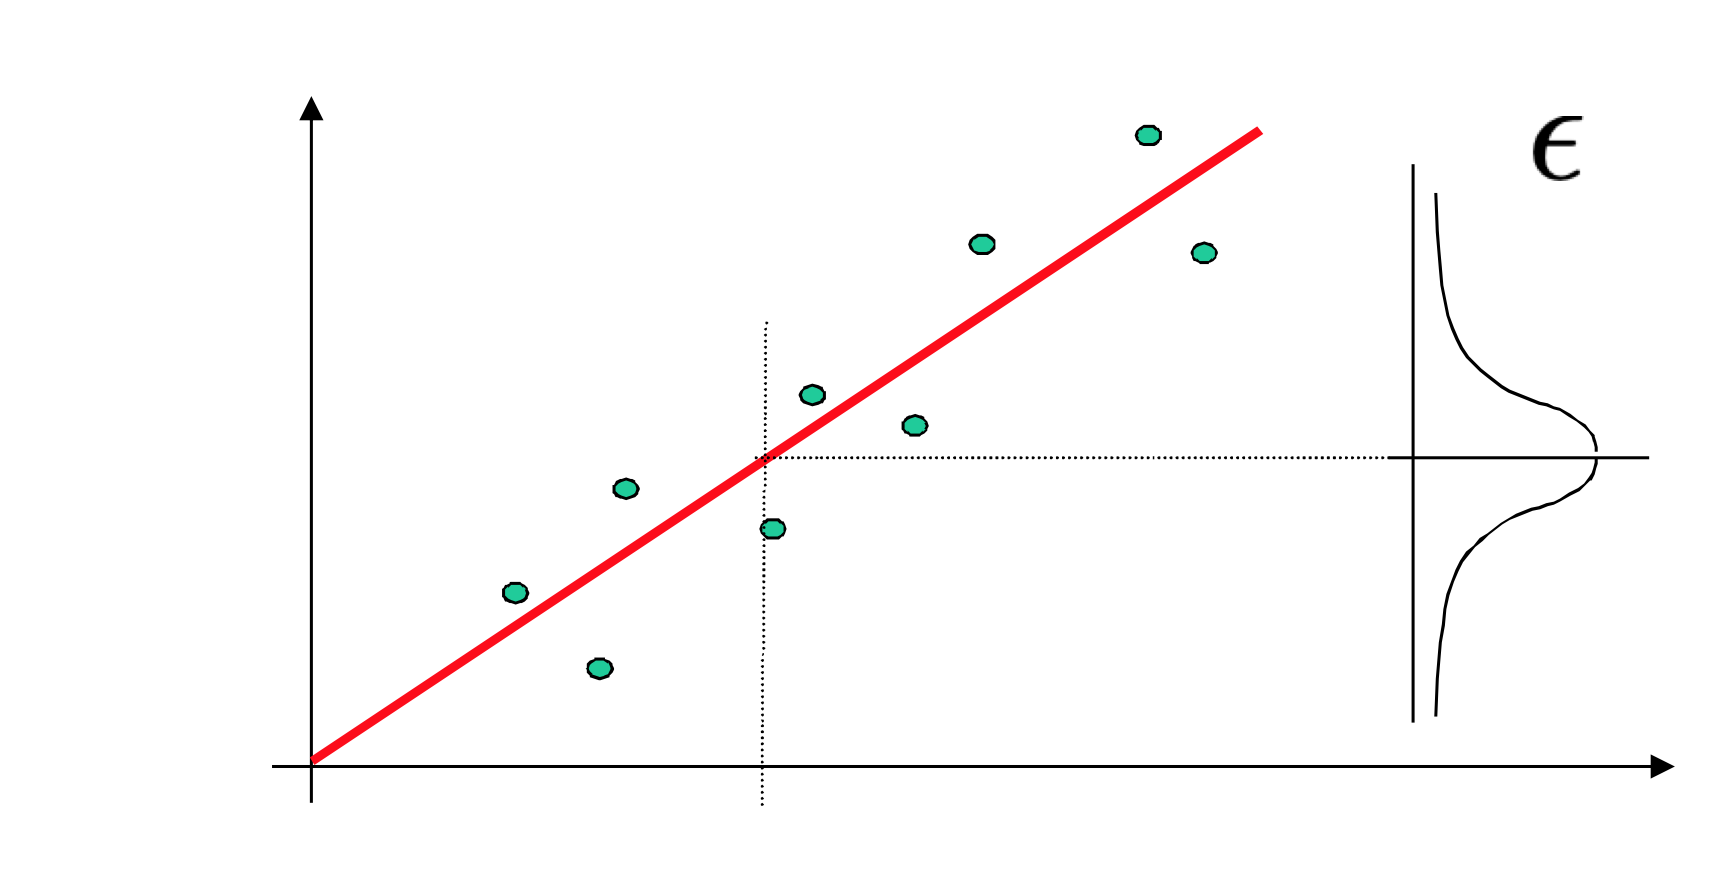
\includegraphics[scale=0.15]{../figures/probabilistic_line.png}}}

\end{frame}





\begin{frame}[fragile]
\frametitle{Maximum Likelihood Estimation}

\begin{itemize}
\item Similar to building deterministic models, probabilistic model parameters need to be tuned/trained
\item \textbf{\textcolor{blue}{Maximum-likelihood estimation (MLE)}} is a method of estimating the parameters of a probabilistic model.
\vspace{8pt}
\uncover<2->{\item Assume \textcolor{blue}{$\boldsymbol{\theta}$}  is a vector of all parameters of the probabilistic model. (e.g. $\boldsymbol{\theta} = \{a_1, \sigma\}$).
\item \textbf{\textcolor{blue}{MLE}} is an extremum
  estimator\footnote{\begin{tiny} ``Extremum estimators are a wide class of estimators for parametric models that are calculated through maximization (or minimization) of a certain objective function, which depends on the data.'' wikipedia.org\end{tiny}} obtained by maximising an objective function of $\boldsymbol{\theta}$}
\end{itemize}

\end{frame}

\begin{frame}[fragile]
\frametitle{Maximum Likelihood Estimation}

\begin{definition}
Assume $f(\theta)$ is an objective function to be optimised (e.g. maximised), the \textcolor{blue}{$arg\,max$} corresponds to the value of $\theta$ that attains the maximum value of the objective function $f$

\vspace{8pt}
\uncover<2->{\begin{equation*}
\hat{\theta} = arg\,max_{\theta} \, f(\theta)
\end{equation*}}
\end{definition}

\begin{itemize}
%\uncover<3->{\item \textbf{\textcolor{red}{Note:}} this is different than maximising the function (i.e. finding the maximum value [$max \, f(\theta)$])}
\uncover<3->{\item  Tuning the parameter is then equal to finding the maximum argument $arg\,max$}

\end{itemize}

\end{frame}


\begin{frame}[fragile]
\frametitle{Maximum Likelihood Estimation - General}

\begin{itemize}
\item Maximum Likelihood Estimation (MLE) is a common method for solving such problems
\begin{align*}
\theta_{MLE} &= arg\,max_\theta \, p(D|\theta)\\
 &= arg\,max_\theta \, \ln p(D|\theta)\\
 &= arg\,min_\theta \, -\ln p(D|\theta)
\end{align*}
\vspace*{-6pt}
\uncover<2->{\begin{block}{MLE Recipe}
\begin{enumerate}
\vspace{6pt}
\uncover<3->{\item Determine $\theta$, $D$ and expression for likelihood $p(D|\theta)$}
\vspace{6pt}
\uncover<4->{\item Take the natural logarithm of the likelihood}
\vspace{6pt}
\uncover<5->{\item Take the derivative of $\ln p(D|\theta)$ w.r.t. $\theta$. If $\theta$ is a multi-dimensional vector, take partial derivatives}
\vspace{6pt}
\uncover<6->{\item Set derivative(s) to 0 and solve for $\theta$}
\end{enumerate}
\end{block}}
\end{itemize}

\end{frame}

%%%%%%%%%%%%%%%%%%%%%%%%%%%%%%%%%%%%%%%%%%%%%%%%%%%%%%%%%%%%%%%%%%%%%%
\begin{titledslide}{Least Squares and MLE for Linear Regression}

  \begin{itemize}
  \item In the case of standard linear regression one can prove that
    the parameters which minimise the squared error are also the MLE
    parameters.
  \item Note that in general the MLE recipe just given will only find
    local maxima of the likelihood (so not necessarily the MLE).
  \item But in the special case of linear regression it does find the MLE.
  \end{itemize}
  
\end{titledslide}

%%%%%%%%%%%%%%%%%%%%%%%%%%%%%%%%%%%%%%%%%%%%%%%%%%%%%%%%%%%%%%%%%%%%%%
\begin{frame}[fragile]
\frametitle{Data Modelling - Deterministic vs Probabilistic}

\begin{itemize}
\item \textbf{\textcolor{blue}{Probabilistic Models}} can tell us \textcolor{red}{more}
\uncover<2->{\item We could use the same MLE recipe to find \textcolor{red}{$\sigma_{ML}$}. This would tell us how uncertain our model is about the data $D$.}
\uncover<3->{\item For example: if we apply this method to two datasets ($D_1$ and $D_2$) what would the parameters $\theta = \{{a_1},\sigma\}$ be?}
\end{itemize}
\uncover<4->{\centerline{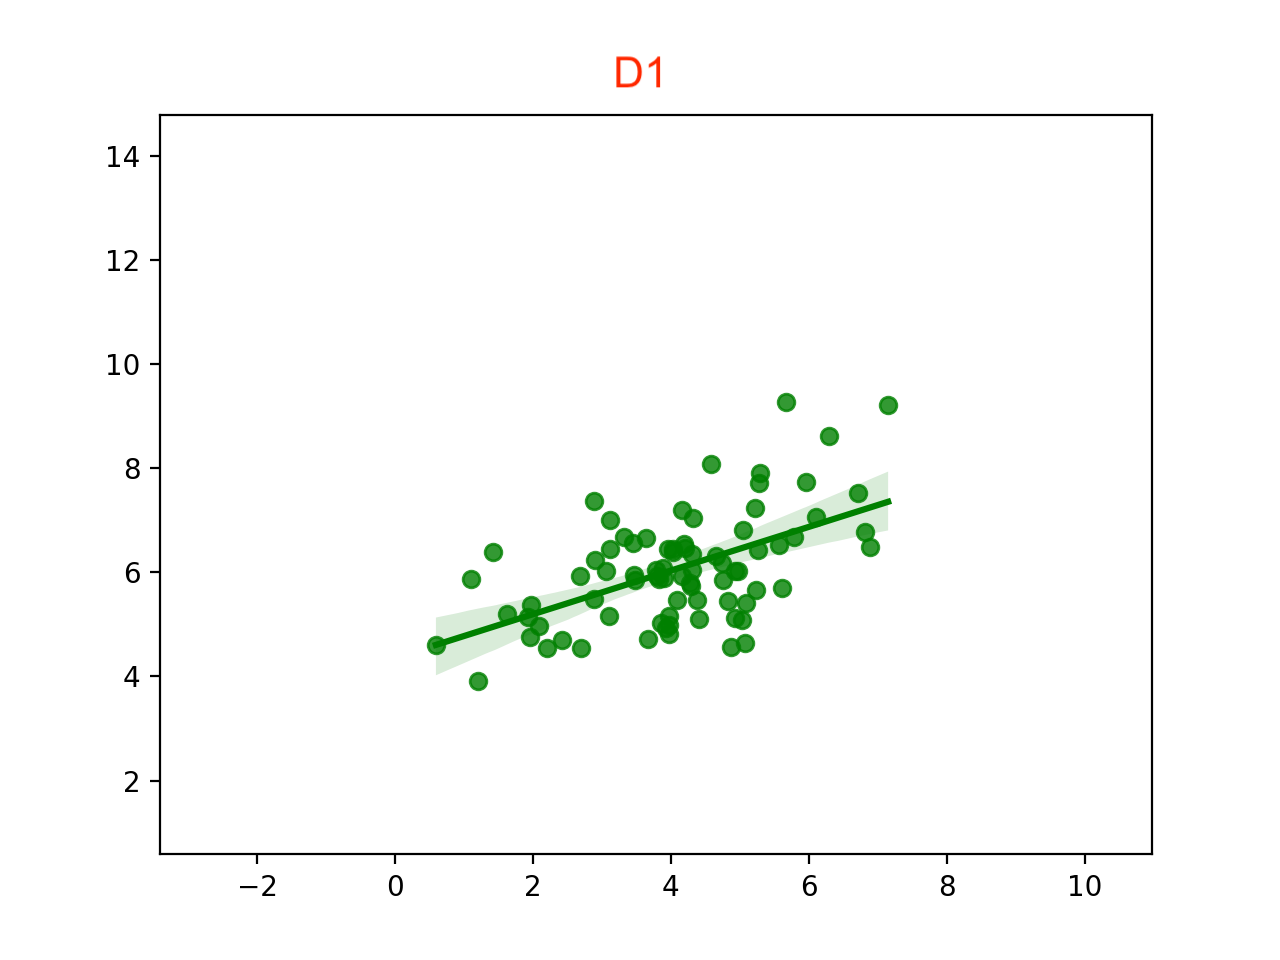
\includegraphics[scale=0.35]{../figures/low_var.png}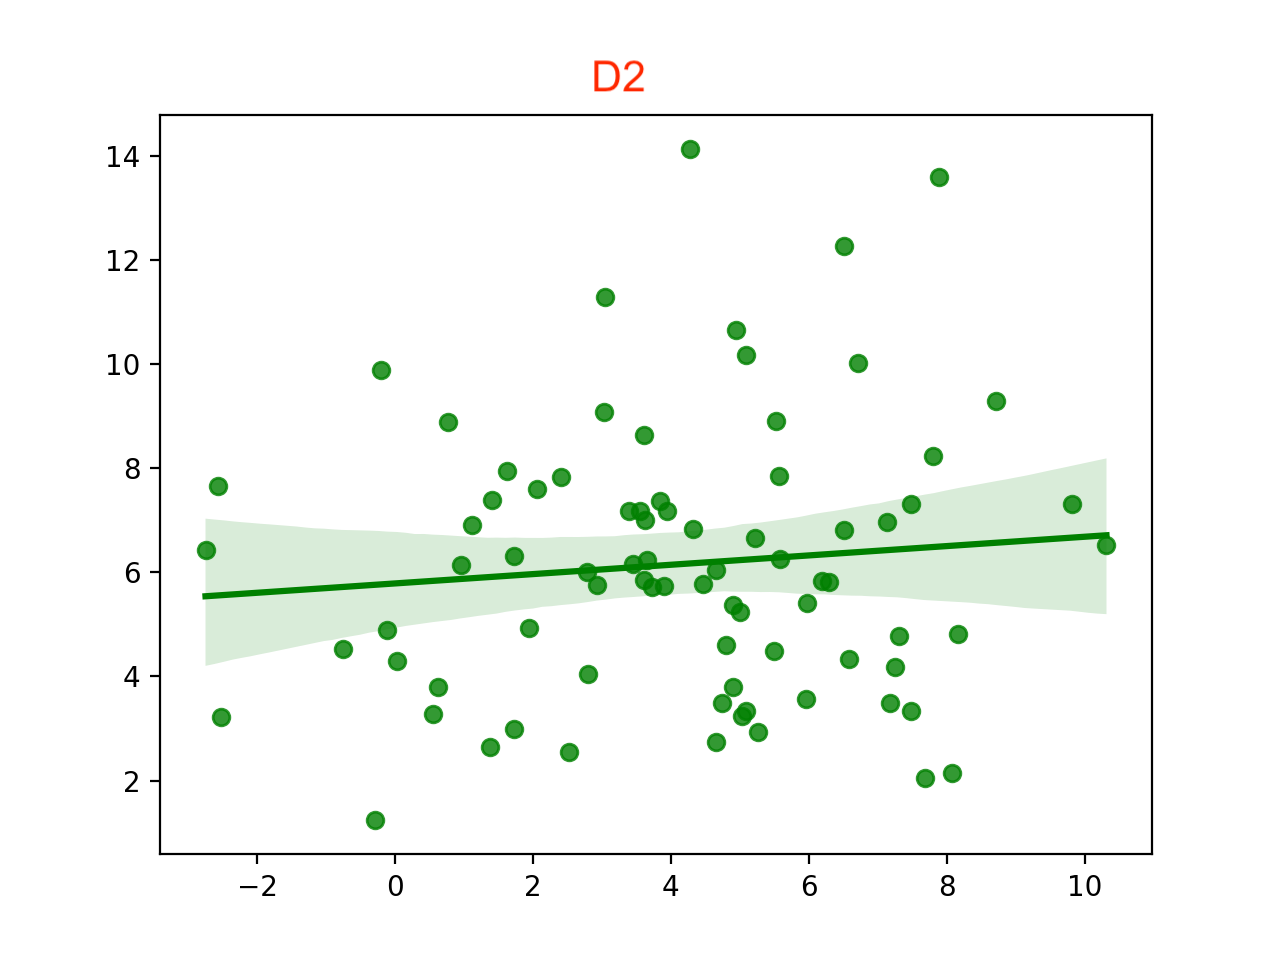
\includegraphics[scale=0.35]{../figures/high_var.png}}}

\uncover<5->{\centerline{${a_1}_{ML}^{D_1} > {a_1}_{ML}^{D_2} \:$ \small{[slope]} and \textcolor{red}{$\: \sigma_{ML}^{D_1} < \sigma_{ML}^{D_2}$ \small{[uncertainty\footnote{The uncertainty ($\sigma$) is represented by the light green bar in the plots. Test it yourself.}]}}}}

\end{frame}


\begin{frame}[fragile]
\frametitle{Textbooks}
We will follow parts of the Chapter 4 and 5 of the Bishop book:
\begin{itemize}
	\item Bishop, C. M., Pattern recognition and machine learning (2006). Available for free \href{https://www.microsoft.com/en-us/research/people/cmbishop/}{\underline{here}.}	\vspace{10pt}
\vspace{10pt}
\end{itemize}
\end{frame}

\begin{frame}[fragile]
\frametitle{Agenda}
	\begin{itemize}
		\item Discriminant functions
		\item Logistic regression			
		% \item Perceptron
		% \item Neural networks (multi-layer perceptron)
		% \begin{itemize}
		% 	\item Architecture
		% 	\item The backpropagation algorithm
		% 	\item Gradient descent
		%\end{itemize}
%		\item Optimising nnets using backprop
%		\item Highly flexible model $\rightarrow$ overfitting: early stopping/drop-out.
%		\item Probabilistic variants [see Bishop]

%		\item Model selection: training/testing, cross-validation
%		\item Parametric vs non-parametric models
%		\item Decision theory (and information theory?)			
	\end{itemize}
See: \begin{small}[Chapter 5, Bishop]\end{small}
\end{frame}



\begin{frame}[fragile]
\frametitle{Classification}

\begin{itemize}
\item It is the classical example of \textbf{supervised learning} \vspace{10pt}
\item Goal: Classify input data into one of $K$ classes \vspace{10pt}
\uncover<2->{\item Model: \emph{Discriminant function}:\vspace{5pt}
	\begin{itemize}
		\item A function that takes an input vector $x$ and assigns it to class $C_k$. 
		For simplicity we will focus on $K=2$ and will first study linear functions (see Bishop for the general cases).
	\end{itemize}}
\end{itemize}

\end{frame}




\begin{frame}[fragile]
\frametitle{Linear discriminant function}

\begin{itemize}
\item The simplest linear discriminant (LD) is $\boxed{y(x) = w_0 + \bm{w^Tx}}$
	\begin{itemize}
		\item \textcolor{darkgray}{where $y$ is used to predicted class $C_k$, $x$ is the input vector (feature values)
		\item $w_0$ is a scalar, which we call \emph{bias}
		\item $w_T$ is our vector of parameters, which we call \emph{weights}}		
	\end{itemize}\vspace{5pt}
\uncover<2->{\item This looks like linear regression! Except the next step...}
\uncover<3->{\item For $K=2$: An input vector $x$ is assigned to class $C_1$ if $y(x) \geq 0$ and to class $C_2$ otherwise.}
\uncover<4->{\item A direct application of least-squares to choose
  $w_0$ and $\mathbf{w}$ does not give great results. See Bishop \S
  4.1.3}
\uncover<5->{\item Instead we can assume the data from each class has
  a Gaussian distribution whose mean is class-specific (but where the
  covariance matrix for each class is the same), use MLE to find parameters
  for each of these Gaussians and finally use Bayes theorem to assign
  classes. See
  \href{https://scikit-learn.org/stable/modules/lda_qda.html}{scikit-learn explanation}.}
\end{itemize}
\end{frame}


\begin{frame}[fragile]
\frametitle{LD and linear separability}

\begin{example}
\emph{Linear separability} is when two sets of points are separable by a line. We generated two sets of points using two Gaussians to illustrate this point, which can easily be fit by a LD. A \emph{decision boundary} is the boundary that separates the two given classes, which our models will try to find.\\	
\centerline{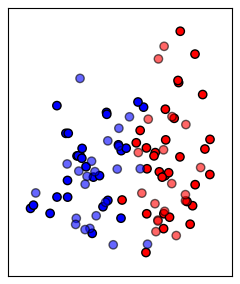
\includegraphics[scale=0.4]{../figures/linear_separable.png}}
\end{example}

\end{frame}


\begin{frame}[fragile]
\frametitle{Linear separability vs nonlinear separability}

\begin{example}
Which datasets \textbf{are} and \textbf{are not} linearly separable\footnote{Example from Sklearn \href{https://scikit-learn.org/stable/auto_examples/classification/plot_classifier_comparison.html}{here}.}? \vspace{5pt}\\	
\centerline{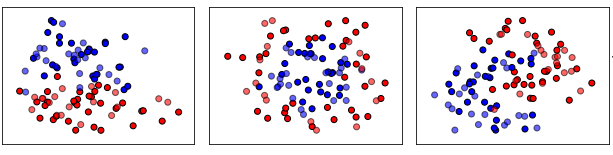
\includegraphics[scale=0.5]{../figures/inputdata.png}}
\end{example}

\uncover<2->{Only the first dataset is linearly separable!}

\end{frame}




\begin{frame}[fragile]
\frametitle{Linear discriminant}

\begin{example}
Using sklearn we fitted a LD to the data: \vspace{5pt}\\	
\centerline{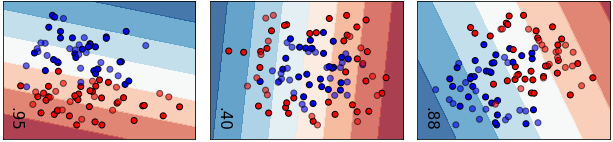
\includegraphics[scale=0.5]{../figures/ld_class.png}}
\end{example}

As expected, the LD model only does a good job in finding a good separation in the first dataset.

\end{frame}





\begin{frame}[fragile]
\frametitle{Logistic regression}

\begin{itemize}
\item We use a logistic function to obtain the probability of class $C_k$: $\boxed{y(\bm{x}) = \sigma(\bm{w^Tx})}$ where $\sigma$ denotes the logistic sigmoid function (s-shaped), for example:
\centerline{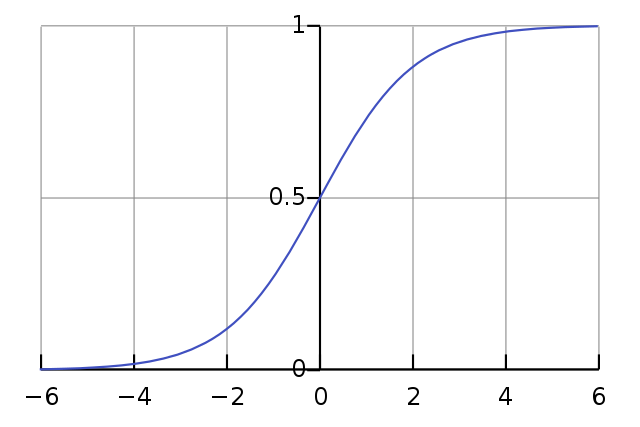
\includegraphics[scale=0.2]{../figures/logistic_function.png}}
\uncover<2->{\item such that when $y \to 0$ we choose class 2 and $y \to 1$ class 1.
\item Taking a probabilistic view: 

$p(C_1|\bm{x}) = y(\bm{x})$, and $p(C_2|\bm{x}) = 1- p(C_1|\bm{x})$.}
\end{itemize}

\end{frame}


\begin{frame}[fragile]
\frametitle{Logistic regression -- maximum likelihood estimation}

Follow MLE recipe:
\begin{enumerate}
	\item Define likelihood: For a dataset $\{x_n, t_n\}$, where the targets $t_n \in \{0,1\}$ we have $p(\bm{t}|\bm{x},\bm{w}) = \mathlarger{\prod_{n=1}^N} y_n^{t_n} (1 - y_n)^{1-t_n}$ where $y_n = p(C_1|x_n)$. \footnote{The exponent selects the probability of the target class (i.e. if $t_n = 1$ we get $y_n$; if $t_n = 0$ we get $1-y_n$).}
\uncover<2->{	\item Take negative logarithm of the likelihood \footnote{Note that we used the logarithm product and power rule.}: $-ln\:p(\bm{t}|\bm{x},\bm{w}) = - \mathlarger{\sum_{n=1}^N}\{t_n ln\:y_n + (1-t_n)ln(1-y_n)\}$}
\uncover<3->{	\item Calculate the derivative w.r.t. the parameters $\bm{w}$:\footnote{This solution makes sense since we want to optimise the difference between the model output $y$ and the desired targets $t$.} \\ $\frac{d\:ln\:p(\bm{t}|\bm{x},\bm{w})}{d \bm{w}} = \mathlarger{\sum_{n=1}^N} (y_n - t_n)x_n$ }
\uncover<4->{	\item Now we can use Eq. above to directly update $\bm{w}$ using the data $x$.}
\end{enumerate}

\end{frame}

\begin{frame}[fragile]
\frametitle{MLE using Gradient Descent}
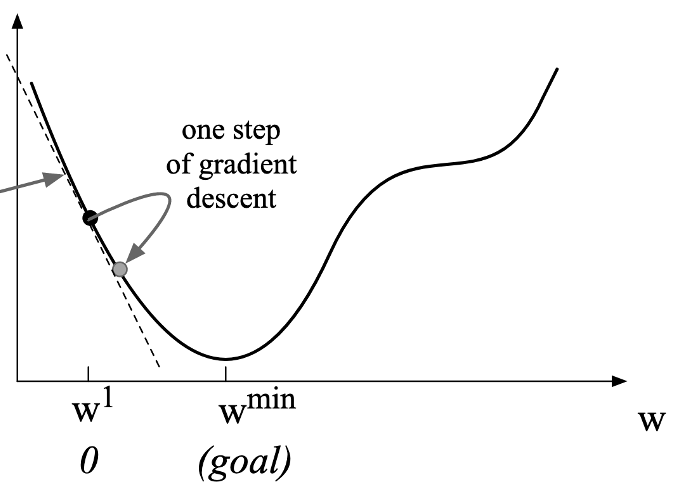
\includegraphics[scale=0.5]{../figures/gradient_descent.png}
\begin{itemize}
\item Start with random weight values 
\item We want to adjust each weight $w$  to minimise negative log likelihood: move downhill to the minimum
\item The derivative represents the slope: $\frac{d\:ln\:p(\bm{t}|\bm{x},\bm{w})}{d \bm{w}} = \mathlarger{\sum_{n=1}^N} (y_n - t_n)x_n$
\item Increase or decrease $w$ by a small amount in the downward direction 
\end{itemize}
\end{frame}


\begin{frame}[fragile]
\frametitle{Logistic regression -- maximum likelihood estimation}

More details on calculating the derivative:
\begin{enumerate}
	\item	From here $-ln\:p(\bm{t}|\bm{x},\bm{w}) = - \mathlarger{\sum_{n=1}^N}\{t_n ln\:y_n + (1-t_n)ln(1-y_n)\}$
\uncover<2->{	\item We get $\mathlarger{\sum_{n=1}^N}\{ - \frac{t_n}{y_n} + \frac{(1-t_n)}{1-y_n}\} \{y_n(1-y_n)\}x_n$ \footnote{We used the chain rule and $d\: ln(x) = 1/x$. We also used the derivative of the sigmoid $d y_n = y(1-y_n)$.}}
\uncover<3->{	\item The above simplifies to $\mathlarger{\sum_{n=1}^N}\{ - t_n (1-y_n) + (1-t_n)y_n\}x_n$}
\uncover<4->{	\item And in turn to $\mathlarger{\sum_{n=1}^N}\{ y_n - t_n \} x_n$ \footnote{You can find the full derivation \href{https://uob-coms30035.github.io/lectures/lect04/CrossEntropy.html}{here}.}}
\end{enumerate}

\end{frame}





\begin{frame}[fragile]
\frametitle{Logistic regression}

\begin{example}
Using sklearn we fitted a logistic regression classifier to the data: \vspace{5pt}\\	
\centerline{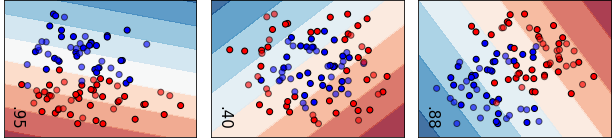
\includegraphics[scale=0.5]{../figures/LR_class.png}}
\end{example}
\small As you can see the results are very similar to LD, but because of probabilistic formulation we have an explicit probability of belonging to one or the other class (not shown); \underline{this can be very useful in real-world applications} (e.g. self-driving cars or cancer detection).
\end{frame}



\begin{frame}[fragile]
\frametitle{Quiz time!}
\centerline{
\includegraphics[scale=0.3]{../figures/BB.png}\vspace{10pt}}
\begin{center}\begin{Large} Go to Blackboard unit page $\gg$ Quizzes $\gg$ Week 1,  Revisiting Regression \end{Large}\end{center}\vspace{10pt}
\centerline{[Should take you less than 5 minutes]}
\end{frame}

\end{document}
